\documentclass[11pt,a4paper]{article}
\usepackage[margin=2.4cm]{geometry}
\usepackage{amsmath,amssymb,amsthm,mathtools}
\usepackage{graphicx,booktabs,xcolor}
\usepackage{tikz}
\usetikzlibrary{arrows.meta,positioning,calc,automata}
\usepackage{algorithm,algpseudocode}
\usepackage[hidelinks]{hyperref}

\definecolor{rl}{HTML}{2471A3}
\newtheorem{theorem}{Theorem}
\newtheorem{proposition}{Proposition}
\newtheorem{lemma}{Lemma}
\newtheorem{corollary}{Corollary}
\theoremstyle{definition}
\newtheorem{definition}{Definition}
\newtheorem{remark}{Remark}

\newcommand{\R}{\mathbb{R}}
\newcommand{\E}{\mathbb{E}}
\newcommand{\Om}{\Omega}
\newcommand{\pos}[1]{\left(#1\right)^{+}}
\DeclareMathOperator*{\argmin}{arg\,min}

\title{\textbf{GRACE}: Goal-Relevant Adaptive Compressed Exchange\\[2pt]
\large Communicating as little as possible, and only what changes a teammate's decision,\\
in teams of memory- and bandwidth-limited agents}
\author{Ropera Labs\\\small Technical report RL-TR-2026-03 \textperiodcentered{} swarm-dil v0.3}
\date{November 2026}

\begin{document}
\maketitle

\begin{abstract}
A team of $N$ agents must travel from a point $A$ to a point $B$ across terrain that none of them knows, with obstacles and radio interference. Each agent sees only through a short vision cone, can remember only a few hundred bytes of map, and talks to teammates over short, fading, shared radio links. We ask which information an agent should transmit, in how many bytes, and how often, so that the team arrives with the least detour per byte spent. Rather than adapting an existing command-and-control protocol, we derive one from the decision problem itself. We show that, under optimistic planning, only obstacle knowledge has decision value (Lemma~\ref{lem:blocked}); that a report saves at most twice the distance the receiver would have flown before seeing the obstacle itself (Proposition~\ref{prop:voi}); that an \emph{ellipse} with the agent and the goal as foci separates relevant from irrelevant knowledge (Lemma~\ref{lem:ellipse}); that the loss probability of $k$ copies over a Gilbert--Elliott link has the closed form $\pi_B\prod_m(\pi_B+\pi_G\lambda^{\tau_m})$ (Proposition~\ref{prop:allLost}), which yields value-proportional redundancy without acknowledgements; and that the byte-optimal tile for what a range sensor actually sees has side $\sqrt{8\,b_{\mathrm{id}}}=4$ (Corollary~\ref{cor:tile}). The resulting protocol, GRACE, runs on board each simulated agent, which receives nothing but its own sensor readings and raw bytes from teammates. In simulation it reaches the detour of exhaustive flooding with several times fewer bytes. All code, data and figures are open and reproducible.
\end{abstract}

\section{Problem and contributions}

\paragraph{Operational setting.} Small autonomous vehicles deployed \emph{on premise}, without cloud or infrastructure, carry little memory and narrow-band radios whose links are short, fade for seconds at a time, are blocked by terrain and are degraded by other emitters. A team crossing unknown terrain can still help itself: an agent that discovers a dead end can spare its followers the detour. The question is \emph{what to say}. Sending everything (flooding) wastes the channel and memory on facts nobody needs; staying silent wastes travel.

\paragraph{Design principle.} We do not copy an existing command-and-control (C2) protocol. We start from the decision each receiver makes (where to move next) and keep only information that can change it, encode it in the fewest bytes that the geometry of sensing allows, and repeat it exactly as often as its value justifies given how the link fades.

\paragraph{Contributions.}
\begin{enumerate}
\item A formal model of on-device agents with a vision cone, bounded memory and a physical radio, in which an agent's software may only use its own sensor readings, proprioception and received bytes (Section~\ref{sec:model}).
\item Decision-relevance results for a team sharing one goal: obstacle-only sufficiency, monotonicity, a tight bound on the value of an obstacle report, the ellipse lemma, the plan-equivalence closure and an ellipse prior with a self-calibrating scale (Sections~\ref{sec:nav}--\ref{sec:voi}).
\item Delivery over bursty links without acknowledgements: the closed-form loss of spaced copies, conditioning that exploits link reciprocity, optimal spacing, and an optimal number of copies that grows only with the logarithm of the value (Section~\ref{sec:channel}).
\item A per-slot selection rule that is exactly optimal for its objective, with a price per byte that traces the bytes-to-detour Pareto front (Section~\ref{sec:select}).
\item A code whose tile size is derived, not chosen, and whose merge is a join-semilattice, so duplicates and reordering are harmless (Section~\ref{sec:code}); and a relevance-aware forgetting rule for bounded memory (Section~\ref{sec:memory}).
\item The GRACE protocol (Algorithm~\ref{alg:grace}) and a simulation study against silence and flooding (Section~\ref{sec:experiments}).
\end{enumerate}

\paragraph{Related work.} Optimistic (``freespace'') replanning is classical in navigation of unknown terrain: D*~\cite{stentz94} and D* Lite~\cite{koenig02}. Occupancy grids go back to~\cite{moravec85}. Value of information is due to Howard~\cite{howard66}. Burst-noise channels are the Gilbert--Elliott model~\cite{gilbert60,elliott63}. Conflict-free replicated data types~\cite{shapiro11} formalise merges that tolerate duplication and reordering. Recent multi-UAV work handles intermittent links by online task allocation~\cite{ccopi}, by predicting missing messages in a learned latent space~\cite{karakasis26}, or by desynchronising broadcasts~\cite{zhao26}. To our knowledge, no prior protocol derives \emph{what} to send, \emph{in how many bytes} and \emph{how many times} from the receivers' navigation decisions under a burst-loss model, with a hard bound on on-board memory.

\section{Model}\label{sec:model}

\subsection{World}
The world is a grid $\Om_n=\{0,\dots,n-1\}^2$ with cell side $c$ metres. A set $O\subset\Om_n$ of cells is blocked; $A,B\in\Om_n\setminus O$ are start and goal. For a set $S$ of cells regarded as blocked, $G(S)$ is the 8-connected graph on $\Om_n\setminus S$ with step costs $1$ (orthogonal) and $\sqrt2$ (diagonal), where a diagonal step is forbidden if either orthogonal cell it passes between is in $S$. We write
\[
d_S(x)=\text{shortest-path cost from }x\text{ to }B\text{ in }G(S),\qquad d^\star=d_O(A).
\]
On the empty grid the octile distance $h(x,y)=\max(|\Delta x|,|\Delta y|)+(\sqrt2-1)\min(|\Delta x|,|\Delta y|)$ is exact; hence for every $S$
\begin{equation}\label{eq:admissible}
h(x,y)\le d_S(x,y).
\end{equation}

\subsection{Agents}
Agent $i\in\{1,\dots,N\}$ starts at $A$ and may move from slot $t_i^0=(i-1)\Delta$ (a staggered launch). Each slot it either holds or commands one 8-connected step; the world executes it if the target cell is free (with the corner rule) and reports success. The agent keeps its position by dead reckoning from $A$.

\paragraph{Vision cone.} With heading $\theta$, range $r$ and half-angle $\alpha$, the agent receives the cells of
\[
\mathcal C(x,\theta)=\{y:\ \|y-x\|\le r,\ \angle(y-x,\theta)\le\alpha\}
\]
that are in line of sight: rays are cast from $x$, and each ray stops at the first blocked cell, which is reported as blocked. Cells behind an obstacle are never seen, so an agent only learns obstacle \emph{surfaces}. Readings are relative offsets $(\Delta x,\Delta y,\text{blocked})$.

\paragraph{Memory.} Map knowledge is a set $K_i\subseteq O$ stored as $4\times4$ tiles of 4 bytes (Section~\ref{sec:code}), at most $M$ tiles. Protocol tables add one byte per (tile, teammate) and a few bytes per teammate (Table~\ref{tab:memory}).

\subsection{Radio}
Positions in metres feed a physical link model (implemented in \texttt{radio.py}, shared with swarm-dil v0.2). The power received by $i$ from $j$ is
\[
P_{ij}=P_{\mathrm{tx}}-L_0-10\,\eta\log_{10}d_{ij}-L_{\mathrm{obs}}\,\#\{\text{obstacles crossed}\}+S_{ij}(t),
\]
with shadowing $S_{ij}(t)=\rho\,S_{ij}(t-1)+\sqrt{1-\rho^2}\,\sigma\,\varepsilon_t$ symmetric in $(i,j)$, so links fade for seconds at a time and are \emph{reciprocal}. Interferers raise the receiver's noise floor; the packet error rate is a logistic function of the SINR; and a receiver that hears more airtime than one slot shares it (contention). For design we abstract each directed link as a two-state Markov chain (Section~\ref{sec:channel}).

\subsection{Information constraint}
\begin{definition}[on-device agent]
The information set of agent $i$ at slot $t$ is
\[
\mathcal I_i(t)=\{\text{its cone readings},\ \text{its move outcomes},\ \text{the bytes it received}\}_{\le t},
\]
plus the pre-launch mission order ($A$, $B$, $N$, its launch slot and the hardware limits). Every quantity an agent computes (position, map, teammates' positions and knowledge, link quality) is a function of $\mathcal I_i(t)$ only.
\end{definition}
In the code this is enforced structurally: the agent module never imports the world or the radio, and a test checks it.

\subsection{Objective}
Let $L_i$ be the distance agent $i$ flies (plus the true remaining distance if it has not arrived at the horizon). The team regret and the cost are
\[
R=\frac1N\sum_{i=1}^N\Big(\frac{L_i}{d^\star}-1\Big),\qquad \mathrm{Bytes}=\sum_i\sum_t|\text{packet}_i(t)|.
\]
We seek protocols on the lower-left of the $(\mathrm{Bytes},R)$ plane, and report the \emph{information efficiency} $\eta=(R_\varnothing-R)/\mathrm{kB}$, the detour removed per kilobyte relative to silence.

\section{Navigation with partial knowledge}\label{sec:nav}

Each agent follows the optimistic policy: it treats unknown cells as free and steps towards the neighbour minimising cost-to-go,
\[
\pi_K(x)=\argmin_{y\in\mathcal N_{G(K)}(x)}\ c(x,y)+d_K(y).
\]

\begin{lemma}[only obstacles matter]\label{lem:blocked}
The action $\pi_K(x)$ depends on the agent's knowledge only through the set $K$ of cells known to be blocked. Learning that a cell is free never changes an action.
\end{lemma}
\begin{proof}
$\pi_K$ is a function of $G(K)$, which is determined by $K$; free and unknown cells are treated identically.
\end{proof}
Consequently free cells are never stored or sent. The saving is large: in open terrain almost every sensed cell is free.

\begin{lemma}[monotonicity]\label{lem:mono}
If $K\subseteq K'$ then $d_K(x)\le d_{K'}(x)$ for all $x$.
\end{lemma}
\begin{proof}
$G(K')$ is a subgraph of $G(K)$; removing vertices cannot shorten a shortest path.
\end{proof}

\begin{remark}[completeness and its loss]
With unbounded memory the optimistic agent reaches $B$ whenever $B$ is reachable: between two discoveries it follows a believed shortest path, and each time that path is invalidated it adds at least one new blocked cell to the finite set $K$~\cite{stentz94,koenig02}. With bounded memory this argument fails: an agent may forget an obstacle, re-plan through it, rediscover it, and cycle. What it forgets therefore matters (Section~\ref{sec:memory}).
\end{remark}

\section{What is worth telling}\label{sec:voi}

Consider a receiver $j$ at $x$ with knowledge $K$, planning along $\pi$ with arc length $s$, and a report of an obstacle piece $a\subseteq O$ that $j$ does not know.

\begin{definition}[ignorance cost]
If $a$ does not meet $\pi$, telling $j$ about $a$ does not change its plan now. If it does, let $q$ be the point of $\pi$ where $j$ would detect $a$ by itself, at arc length $\ell$. Without the report, $j$ flies to $q$ and then replans; with it, it replans at once. The saving, measured in the knowledge $K\cup a$, is
\[
W=\ell+d_{K\cup a}(q)-d_{K\cup a}(x).
\]
\end{definition}

\begin{proposition}[value of an obstacle report]\label{prop:voi}
$0\le W\le 2\ell$. If $j$ detects $a$ when it comes within path distance $r$ of the first cell of $a$ on $\pi$, at arc length $s_a$, then
\[
0\le W\le 2\pos{s_a-r}.
\]
The upper bound is attained when the only way to $B$ is back through $x$ (a dead end).
\end{proposition}
\begin{proof}
The prefix of $\pi$ from $x$ to $q$ avoids $K$ and, by definition of $q$, does not meet $a$; it is therefore a path of length $\ell$ in $G(K\cup a)$, and so is its reverse. Going from $x$ to $B$ through $q$ gives $d_{K\cup a}(x)\le\ell+d_{K\cup a}(q)$, hence $W\ge0$. Going from $q$ back to $x$ and then to $B$ gives $d_{K\cup a}(q)\le\ell+d_{K\cup a}(x)$, hence $W\le2\ell$. With the detection rule, $\ell=\pos{s_a-r}$. In a dead end every path from $q$ to $B$ passes through $x$, so the second inequality is an equality.
\end{proof}

The bound says something useful about \emph{whom} to tell: an obstacle close ahead of a teammate is worth nothing, because the teammate is about to see it; an obstacle far ahead, especially the bottom of a pocket, is worth up to twice its distance.

\begin{lemma}[ellipse]\label{lem:ellipse}
Let $D=d_K(x)$. Every cell $y$ on an optimistic plan from $x$ satisfies $h(x,y)+h(y,B)\le D$. Equivalently, a cell outside the octile ellipse
\[
\mathcal E(x,B,D)=\{y:\ h(x,y)+h(y,B)\le D\}
\]
cannot lie on the current plan.
\end{lemma}
\begin{proof}
For $y$ on a shortest path, $D=d_K(x,y)+d_K(y)$. By \eqref{eq:admissible}, $d_K(x,y)\ge h(x,y)$ and $d_K(y)\ge h(y,B)$.
\end{proof}

\begin{figure}[t]\centering
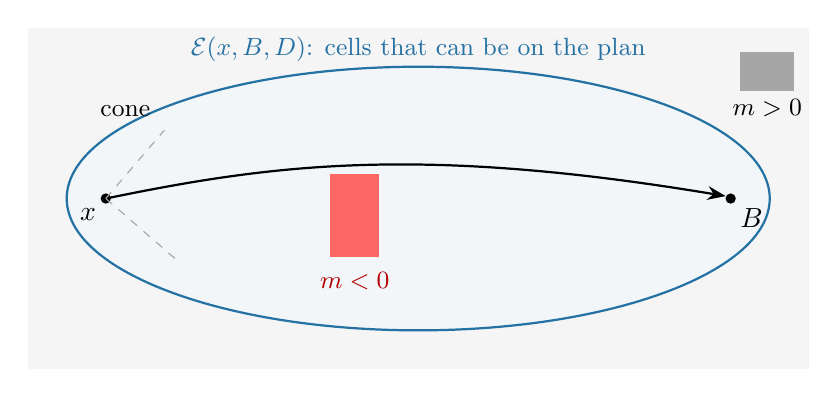
\begin{tikzpicture}[scale=0.62]
  \fill[gray!8] (0,0) rectangle (16,7);
  \draw[rl,thick,fill=rl!6] (8,3.5) ellipse (7.2 and 2.7);
  \node[rl] at (8,6.55) {\small $\mathcal E(x,B,D)$: cells that can be on the plan};
  \fill[black] (1.6,3.5) circle (3pt) node[below left] {$x$};
  \fill[black] (14.4,3.5) circle (3pt) node[below right] {$B$};
  \draw[thick,->,>=Stealth] (1.6,3.5) .. controls (5,4.2) and (8,4.6) .. (14.3,3.55);
  \fill[red!60] (6.2,2.3) rectangle (7.2,4.0); \node[red!70!black] at (6.7,1.8) {\small $m<0$};
  \fill[gray!70] (14.6,5.7) rectangle (15.7,6.5); \node at (15.15,5.35) {\small $m>0$};
  \draw[gray!70,dashed] (1.6,3.5) -- (2.8,4.9); \draw[gray!70,dashed] (1.6,3.5) -- (3.1,2.2);
  \node at (2.0,5.3) {\small cone};
\end{tikzpicture}
\caption{Lemma~\ref{lem:ellipse}. An obstacle tile with positive margin $m=\min_{y}\big[h(x,y)+h(y,B)\big]-d_K(x)$ (grey) cannot touch the current plan; it is the first candidate to forget. Tiles inside the ellipse (red) may.}
\label{fig:ellipse}
\end{figure}

\begin{corollary}[safe forgetting]\label{cor:forget}
Forgetting a tile of positive margin does not change the current plan.
\end{corollary}
\begin{proof}
After forgetting, the cells $y$ of the tile become passable in the agent's belief, but by \eqref{eq:admissible} any path through such a $y$ costs at least $h(x,y)+h(y,B)>D$. The old plan, of cost $D$, is still available and still strictly cheaper than any path through the tile, so it remains optimal.
\end{proof}

A sender does not know the receiver's knowledge. It predicts it from what it believes the team shares (Section~\ref{sec:channel}) and then reasons about which of its own tiles the receiver's plan will run into, \emph{including after the receiver reroutes}.

\begin{definition}[plan-equivalence closure]\label{def:closure}
Let $K^0$ be the knowledge the sender believes $j$ has, and $K_i$ the sender's. Set $P^m=\{a\in K_i\setminus K^m:\ a\cap\pi(K^m)\ne\varnothing\}$ and $K^{m+1}=K^m\cup P^m$. Each tile $a\in P^m$ is valued at $2\pos{s_a-r}$, measured on $\pi(K^m)$.
\end{definition}

\begin{proposition}\label{prop:closure}
The closure stops after at most $|K_i\setminus K^0|$ rounds, and at that point $j$'s predicted plan crosses no obstacle the sender knows of: delivering $\bigcup_mP^m$ would make $j$'s plan consistent with all of the sender's knowledge.
\end{proposition}
\begin{proof}
Every round that does not stop adds at least one tile of the finite set $K_i\setminus K^0$. It stops exactly when $P^m=\varnothing$.
\end{proof}
GRACE truncates the closure at four rounds.

Tiles off every predicted plan may still matter later, when the receiver's believed cost rises as it discovers obstacles the sender does not know.

\begin{proposition}[ellipse prior]\label{prop:prior}
Let $m_j(a)$ be the margin of tile $a$ with respect to $j$ (Lemma~\ref{lem:ellipse} with $x=x_j$, $D=d_{K^0}(x_j)$). If $j$'s believed cost-to-go from $x_j$ later rises by $\Delta\ge0$, then $a$ can be on a plan from $x_j$ only if $\Delta\ge m_j(a)$. If $\Delta\sim\mathrm{Exp}(\mu)$,
\[
\Pr[a\text{ on a future plan from }x_j]\le e^{-\pos{m_j(a)}/\mu}.
\]
\end{proposition}
\begin{proof}
Apply Lemma~\ref{lem:ellipse} with $D+\Delta$ in place of $D$; the exponential tail gives the bound.
\end{proof}
The scale $\mu$ is not a tuning knob: each agent estimates it from its own experience as the inflation of its own belief, $\hat\mu=\max\{1,\ L_i+d_{K_i}(x_i)-h(A,B)\}$, the extra cost that obstacles have revealed so far on this mission. The value GRACE assigns to tile $a$ for teammate $j$ is therefore
\[
V_j(a)=\max\Big\{\,2\pos{s_a-r}\ \text{if }a\in\textstyle\bigcup_mP^m,\ \ e^{-\pos{m_j(a)}/\hat\mu}\,2\pos{h(x_j,a)-r}\Big\}.
\]

\section{Delivering without acknowledgements}\label{sec:channel}

Acknowledgements cost bytes and are lost too. Instead, each sender keeps a belief $u_j(a)$ that teammate $j$ does \emph{not} know its current version of tile $a$, and lowers it every time it sends the tile.

\paragraph{Link abstraction.} The directed link $i\to j$ is a Gilbert--Elliott chain~\cite{gilbert60,elliott63} with a good state $G$ (delivers) and a bad state $B$ (loses), $p=\Pr[G\to B]$, $q=\Pr[B\to G]$ per slot,
\[
\pi_B=\frac{p}{p+q},\qquad \pi_G=1-\pi_B,\qquad \lambda=1-p-q\in(-1,1).
\]
The mean outage lasts $1/q$ slots and $\lambda$ measures how long the link remembers its state.

\begin{figure}[h]\centering
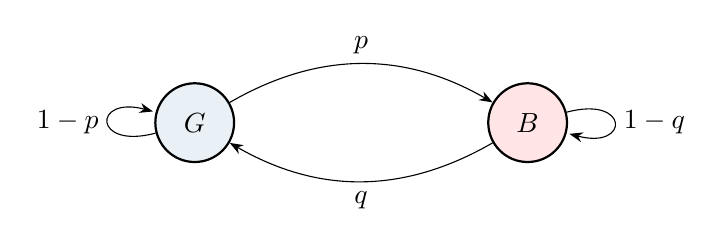
\begin{tikzpicture}[->,>=Stealth,node distance=3.2cm,every state/.style={minimum size=1cm,thick}]
\node[state,fill=rl!10] (G) {$G$};
\node[state,fill=red!10,right=of G] (B) {$B$};
\path (G) edge[bend left] node[above] {$p$} (B)
      (B) edge[bend left] node[below] {$q$} (G)
      (G) edge[loop left] node {$1-p$} ()
      (B) edge[loop right] node {$1-q$} ();
\end{tikzpicture}
\caption{Two-state abstraction of a fading link: $G$ delivers, $B$ loses.}
\end{figure}

\begin{proposition}[conditional state after $\tau$ slots]\label{prop:cond}
\[
\Pr[B_{t+\tau}\mid B_t]=\pi_B+\pi_G\lambda^\tau,\qquad \Pr[B_{t+\tau}\mid G_t]=\pi_B\big(1-\lambda^\tau\big).
\]
\end{proposition}
\begin{proof}
The transition matrix $P=\begin{psmallmatrix}1-p&p\\q&1-q\end{psmallmatrix}$ has eigenvalues $1$ and $\lambda$, and $P^\tau=\mathbf 1\pi^\top+\lambda^\tau(I-\mathbf 1\pi^\top)$. Reading off the entries gives both identities.
\end{proof}

\begin{proposition}[loss of spaced copies]\label{prop:allLost}
If $k$ copies are sent at slots separated by gaps $\tau_1,\dots,\tau_{k-1}$, starting from the stationary distribution,
\[
\Pr[\text{all }k\text{ lost}]=\pi_B\prod_{m=1}^{k-1}\big(\pi_B+\pi_G\lambda^{\tau_m}\big).
\]
\end{proposition}
\begin{proof}
All copies are lost if and only if the chain is in $B$ at every sending slot. By the Markov property this probability is $\pi_B$ times the product of the conditional probabilities of Proposition~\ref{prop:cond}.
\end{proof}

\begin{corollary}[spacing]\label{cor:spacing}
Copies spaced by $\tau\ge\ln\!\big(\varepsilon\pi_B/\pi_G\big)/\ln\lambda$ are lost together with probability at most $(1+\varepsilon)$ times that of independent copies. With bursty links ($\lambda$ close to 1), back-to-back repetition is almost useless: two copies one slot apart are lost together with probability close to $\pi_B$, not $\pi_B^2$.
\end{corollary}
\begin{proof}
By Proposition~\ref{prop:cond}, $\pi_B+\pi_G\lambda^\tau\le(1+\varepsilon)\pi_B$ if and only if $\lambda^\tau\le\varepsilon\pi_B/\pi_G$; take logarithms with $0<\lambda<1$.
\end{proof}

\paragraph{Conditioning on ignorance.} The sender wants the probability that the \emph{next} copy is lost given that $j$ still does not know the tile. That event means every earlier copy was lost, so the link was in $B$ at the last copy, at slot $t_1$. If, after that, the sender heard $j$ (at slot $t_h>t_1$), reciprocity says the link was in $G$ at $t_h$. Hence the loss probability of a copy sent now is
\begin{equation}\label{eq:beta}
\beta_j(a,t)=\begin{cases}\pi_B+\pi_G\lambda^{\,t-t_1}&\text{if }t_1>t_h,\\[2pt] \pi_B\big(1-\lambda^{\,t-t_h}\big)&\text{otherwise,}\end{cases}
\end{equation}
and after sending, $u_j(a)\leftarrow u_j(a)\,\beta_j(a,t)$. Two consequences follow without any extra rule: a tile just sent is not worth repeating until the burst is likely over, and the best moment to send is right after hearing the receiver.

\paragraph{Estimating the link on board.} Each packet carries a one-byte sequence number. From the gaps, the receiver counts messages received and expected from each teammate and keeps the Beta--Bernoulli estimate $\hat q_j=(n_{\mathrm{rx}}+1)/(n_{\mathrm{exp}}+2)$, so $\hat\pi_B=1-\hat q_j$; by reciprocity it uses it for its own link to $j$. The memory $\lambda$ is a design constant calibrated to the shadowing correlation of the radio ($\lambda=0.9$).

\begin{proposition}[how many copies]\label{prop:kstar}
For one tile of value $v$ to one receiver, with cost $c$ per copy and $\rho=\Pr[\text{loss}\mid\text{previous copy lost}]$, the $m$-th copy is worth $v(1-\pi_B)$ for $m=1$ and $v\,\pi_B\rho^{m-2}(1-\rho)$ for $m\ge2$. Sending while a copy is worth at least $c$ gives
\[
k^\star=\begin{cases}0&v(1-\pi_B)<c,\\ 1+\pos{\Big\lfloor\dfrac{\ln\big(c/(v\,\pi_B(1-\rho))\big)}{\ln\rho}\Big\rfloor+1}&\text{otherwise.}\end{cases}
\]
\end{proposition}
Redundancy thus grows only with $\log v$: important facts are repeated a few more times, and trivial ones are sent once or never. The test suite checks $k^\star$ against brute force, and Figure~\ref{fig:theory} checks Proposition~\ref{prop:allLost} against Monte Carlo.

\section{Choosing what to send}\label{sec:select}

In each slot an agent may broadcast one message of at most $b$ bytes: a 4-byte header and up to $\lfloor(b-4)/4\rfloor$ tiles. The expected value of including tile $a$ is
\[
g(a)=\sum_{j\in\mathcal N_i(t)}V_j(a)\,u_j(a)\,\big(1-\beta_j(a,t)\big),
\]
where $\mathcal N_i(t)$ are the teammates heard recently.

\begin{theorem}[per-slot optimality]\label{thm:select}
Among all messages of the slot, the one that maximises expected delivered value minus $\kappa$ per byte contains exactly the tiles with the largest $g(a)$ among those with $g(a)\ge 4\kappa$, up to the size limit.
\end{theorem}
\begin{proof}
With indicator $x_a\in\{0,1\}$ for including tile $a$, the objective $\sum_a x_a\,(g(a)-4\kappa)$ is linear and separable, and the size limit is a cardinality constraint, since all tiles have the same size. Taking the largest positive terms is optimal.
\end{proof}
The price $\kappa$ (detour cells a byte must save) is the Lagrange multiplier of the byte budget: sweeping it traces the protocol's bytes--detour front. Across slots, the multiplicative update of $u$ makes the sequence of copies of a tile follow the rule of Proposition~\ref{prop:kstar}. The header doubles as a heartbeat, sent at least every 5 slots, so that teammates and link estimates stay current.

\section{The code: what to put in each byte}\label{sec:code}

By Lemma~\ref{lem:blocked} only blocked cells are encoded. A tile of side $s$ is sent as a 2-byte identifier $(t_x,t_y)$ and an $s^2$-bit mask of blocked cells.

\begin{lemma}[tiles touched]\label{lem:tiles}
A $w\times h$ block of cells placed at a uniformly random offset touches on average exactly
\[
\E[\#\text{tiles}]=\frac{w+s-1}{s}\cdot\frac{h+s-1}{s}.
\]
\end{lemma}
\begin{proof}
Along one axis an interval of $w$ cells starting at offset $o\in\{0,\dots,s-1\}$ touches $\lceil(o+w)/s\rceil$ tiles, and $\frac1s\sum_{o=0}^{s-1}\lceil(o+w)/s\rceil=(w+s-1)/s$. The axes are independent.
\end{proof}

\begin{corollary}[optimal tile for what is sensed]\label{cor:tile}
A range sensor with line of sight reveals obstacle surfaces, which are sets one cell thick ($h=1$). Per sensed cell, a long surface then costs $(b_{\mathrm{id}}+s^2/8)/s$ bytes, which is minimised at
\[
s^\star=\sqrt{8\,b_{\mathrm{id}}}=4\quad(b_{\mathrm{id}}=2),
\]
giving $1$ byte per cell, half the cost of listing cells. For filled areas larger tiles would be better; the geometry of sensing, not convenience, fixes the tile at $4\times4$.
\end{corollary}

\paragraph{Merging.} Tiles merge by bitwise \textsc{or}. This is the join of a semilattice: idempotent, commutative and associative. Duplicates, reordering and relaying through any number of teammates therefore never corrupt knowledge~\cite{shapiro11}, which is exactly what an acknowledgement-free broadcast over lossy links needs.

\begin{table}[h]\centering\small
\begin{tabular}{lll}
\toprule
Field & Bytes & Content\\\midrule
header & 4 & sender, sequence number, $x$, $y$\\
tile & 4 & $t_x$, $t_y$, 16-bit blocked mask\\
raw cell (baseline only) & 2 & $x$, $y$\\\bottomrule
\end{tabular}
\caption{Wire format. Grids up to $255\times255$ cells.}
\end{table}

\section{Bounded memory}\label{sec:memory}

When an agent holds more than $M$ tiles, GRACE forgets the tile with the largest margin (Corollary~\ref{cor:forget}): the one furthest outside the ellipse between the agent and the goal. As the agent advances, the ellipse shrinks, so memory naturally concentrates on what still lies between the agent and $B$. The baseline forgets the oldest tile (FIFO).

\begin{table}[h]\centering\small
\begin{tabular}{lll}
\toprule
Structure & Size & Note\\\midrule
map & $4M$ B & tiles\\
delivery beliefs $u_j(a)$ & $M\cdot N$ B & quantised to one byte\\
teammate table & $\approx 6N$ B & position, last heard, sequence counters\\
\bottomrule
\end{tabular}
\caption{On-board memory of a GRACE agent.}
\label{tab:memory}
\end{table}

\section{The protocol}

\begin{algorithm}[h]
\caption{GRACE, one slot of agent $i$ (all quantities are functions of $\mathcal I_i(t)$)}\label{alg:grace}
\begin{algorithmic}[1]
\State \textbf{observe}: add the blocked cells of the cone to their tiles; on any change set $u_j(a)\gets1$ for all $j$
\State \textbf{receive}: for each packet, update the teammate's position, last-heard slot and $\hat q_j$; merge tiles by \textsc{or}; if the sender's tile covers mine, $u_{\text{sender}}(a)\gets0$
\State \textbf{forget}: while more than $M$ tiles, drop the tile of largest margin
\State \textbf{select}: predict the shared map (tiles with $\max_ju_j\le\tfrac12$); compute $V_j(a)$ by the closure and the ellipse prior, $\beta_j(a,t)$ by \eqref{eq:beta}, and $g(a)$
\State \textbf{send} the top tiles with $g\ge4\kappa$ (Theorem~\ref{thm:select}), or a header if a heartbeat is due; update $u_j(a)\gets u_j(a)\beta_j(a,t)$
\State \textbf{move}: one step of $\pi_{K_i}$
\end{algorithmic}
\end{algorithm}

\paragraph{Cost.} Each cost-to-go field is a Dijkstra search on $n^2$ cells. Prediction needs one shared field plus at most four per teammate in range, every slot. That is light for a microcontroller at $n=48$ and is the first thing to optimise for larger grids, for instance by recomputing only when the shared map or a teammate's position changes.

\section{Experiments}\label{sec:experiments}

\paragraph{Setup.} Grid $48\times48$ with 5 m cells; 10 random blocks and 4 L-shaped pockets that open towards $A$ (dead ends), regenerated until $B$ is reachable; $N=8$ agents launched every 12 s; vision cone $r=5$ cells, $\alpha=60^\circ$; radio at $-16$ dBm (50\,\% delivery at about 60 m in the open), $\pm20$ dB per obstacle, shadowing $\sigma=4$ dB with $\rho=0.9$, 9.6 kbit/s shared channel; 600 s horizon. Every agent runs its protocol internally (Section~\ref{sec:model}). Each point averages 20 random terrains (seeds), and all protocols see the same terrains. Error bars are one standard error.

\paragraph{Protocols.} \emph{Silence}; \emph{raw-cell flooding} and \emph{tile flooding}, which send, newest first and round robin, as many known blocked cells (2 B) or tiles (4 B) as the per-slot budget allows; \emph{GRACE} with price $\kappa$; and two ablations: GRACE without goal relevance (every unknown tile is worth 1) and GRACE without the loss model ($\beta=0$, so each tile is sent once).

\begin{figure}[t]\centering
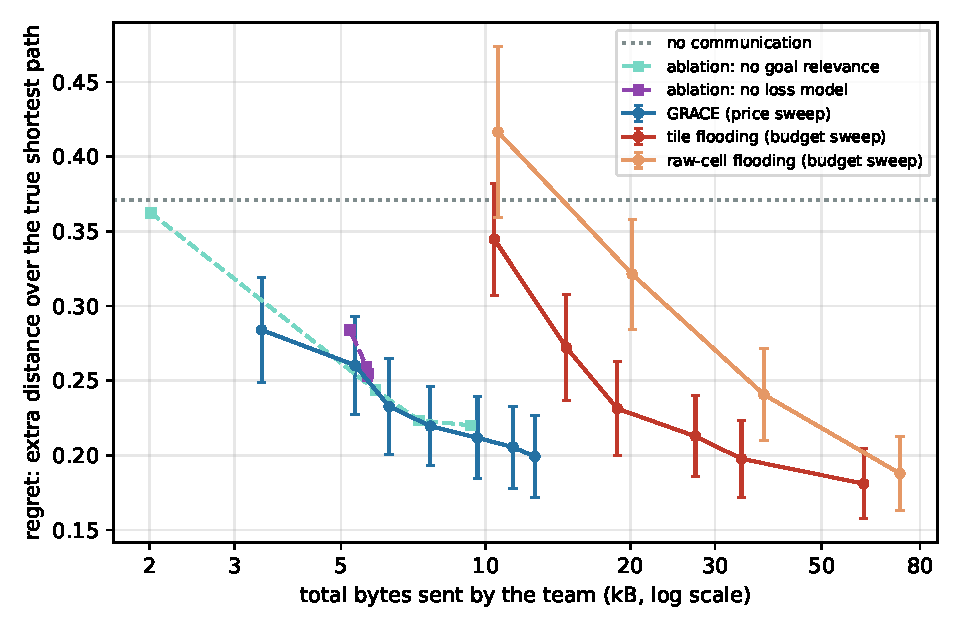
\includegraphics[width=0.72\linewidth]{fig/pareto.pdf}
\caption{Bytes against detour. Each curve sweeps its knob: price for GRACE, per-slot budget for flooding.}
\label{fig:pareto}
\end{figure}

\paragraph{Bytes for the same detour (Figure~\ref{fig:pareto}).} Silence costs a mean regret of $0.371$. GRACE matches the regret of tile flooding with \textbf{2.9--3.3$\times$ fewer bytes}: paired over seeds, GRACE at $\kappa=0.2$ against flooding at 24 B/slot differs by $-0.001\pm0.013$ in regret, with $3.1\times$ fewer bytes (9.6 against 27.3 kB). Against raw-cell flooding the saving is about $6\times$, as Corollary~\ref{cor:tile} predicts for the code alone combined with the scheduling. The information efficiency $\eta$ (regret removed per kB) is $0.013$--$0.026$ for GRACE against $0.002$--$0.007$ for tile flooding. The lowest regret is reached by flooding at 64 B/slot ($0.181$, 61 kB); GRACE's best is $0.199$ with $5.1\times$ fewer bytes, a paired difference of $0.018\pm0.010$. Raw-cell flooding with a small budget ($0.417$) is no better than silence: partial, unprioritised obstacle knowledge can push optimistic planners into unexplored pockets.

\paragraph{What each component buys.} Without the loss model, the protocol sends each tile once and never repairs a loss: its curve stalls at a regret of $0.253$ whatever the price, while GRACE keeps converting bytes into lower regret down to $0.199$. Without goal relevance, the curve lies on GRACE's own front within error bars in this scenario. We therefore cannot claim a measurable benefit of goal relevance \emph{for transmission} here: with a short convoy along similar routes, most tiles are relevant to someone. Relevance does matter for memory (next paragraph).

\begin{figure}[t]\centering
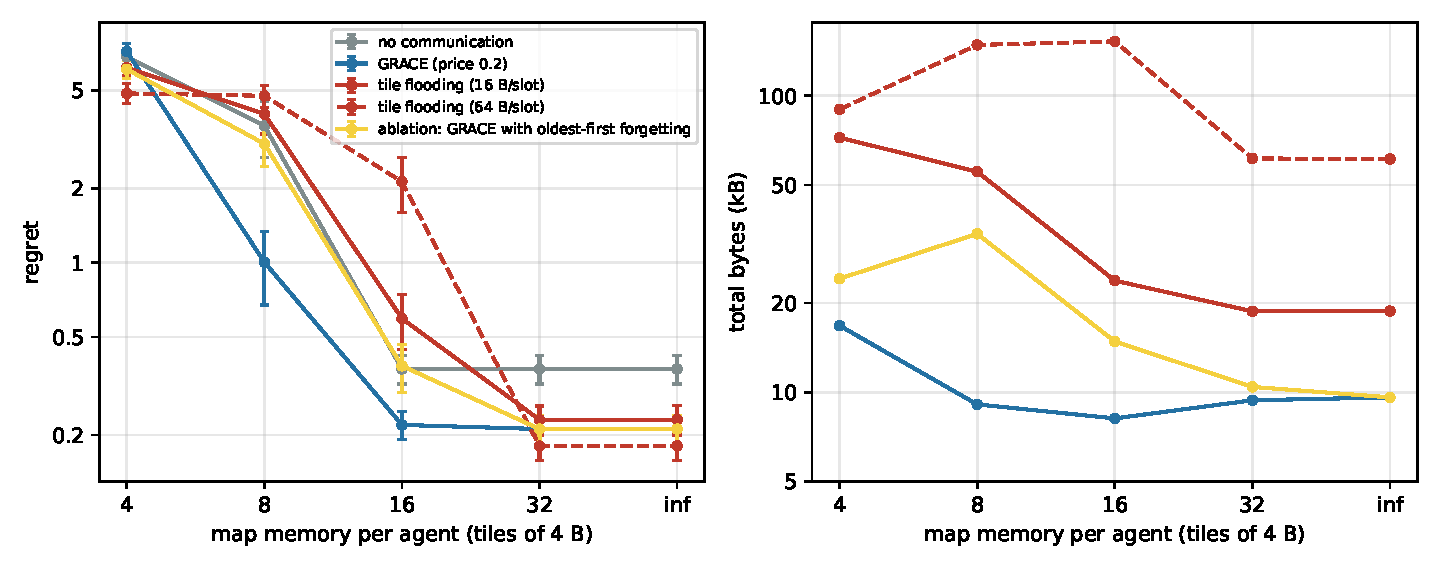
\includegraphics[width=\linewidth]{fig/memory.pdf}
\caption{Bounded map memory. Left: regret (log scale). Right: bytes. One tile is 4 bytes.}
\label{fig:memory}
\end{figure}

\paragraph{Bounded memory (Figure~\ref{fig:memory}).} With 16 tiles (64 bytes of map memory) per agent, GRACE stays at its unlimited-memory regret ($0.220$ against $0.212$) with full arrival. With the same memory, tile flooding degrades from $0.231$ to $0.594$ (16 B/slot) and from $0.181$ to $2.13$ (64 B/slot), worse than silence, with 18\,\% of agents not arriving: incoming tiles that do not matter evict the ones that do, and agents loop. Replacing ellipse-margin forgetting by oldest-first forgetting in GRACE raises the regret to $0.382$, so the relevance-aware memory rule of Corollary~\ref{cor:forget} accounts for most of the difference. At 8 tiles, GRACE keeps 89\,\% of agents arriving, against 60\,\% for silence and 43--59\,\% for flooding. At 4 tiles every protocol fails, because an agent cannot even hold the pocket it is standing in.

\begin{figure}[t]\centering
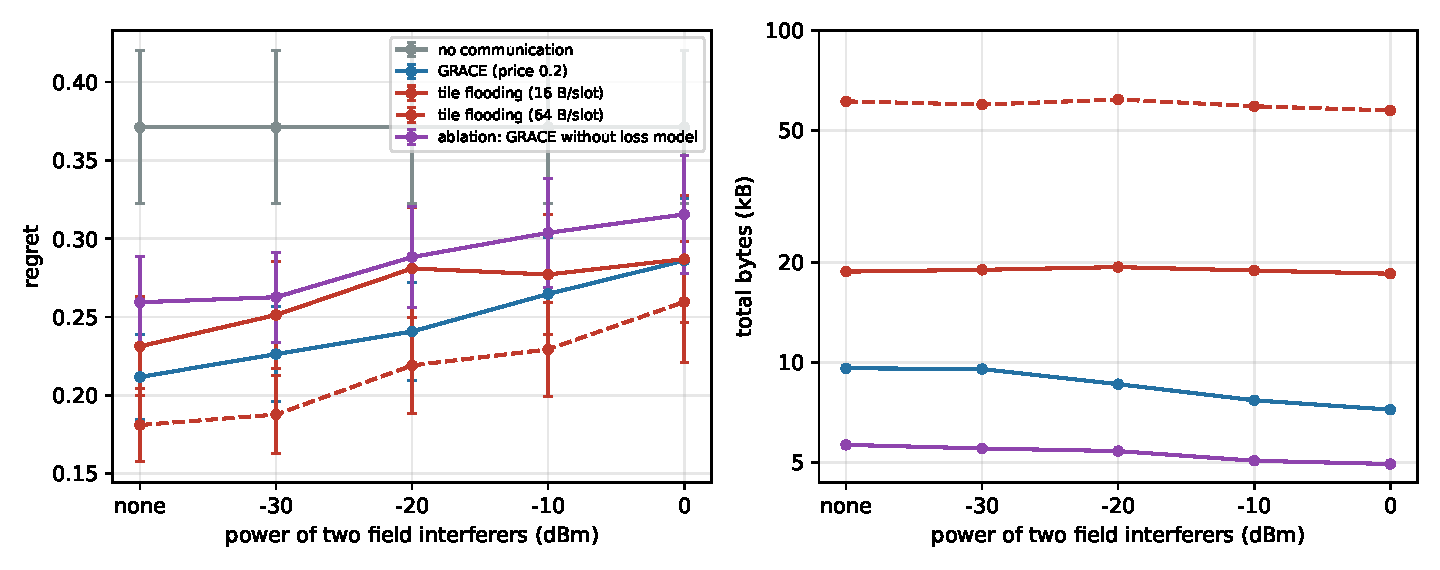
\includegraphics[width=\linewidth]{fig/interference.pdf}
\caption{Two field interferers near the middle of every route, increasing power.}
\label{fig:interference}
\end{figure}

\paragraph{Interference (Figure~\ref{fig:interference}).} As the interferers grow from off to 0 dBm, every protocol loses part of its benefit. GRACE's regret rises from $0.212$ to $0.286$, which equals tile flooding at 16 B/slot ($0.287$) with $2.6\times$ fewer bytes. Without being told anything, GRACE \emph{spends less} as the channel degrades (9.6 to 7.2 kB): fewer teammates are heard and \eqref{eq:beta} makes copies into bad links look less valuable. Flooding keeps spending the same. The ablation without the loss model is worse at every interference level.

\begin{figure}[t]\centering
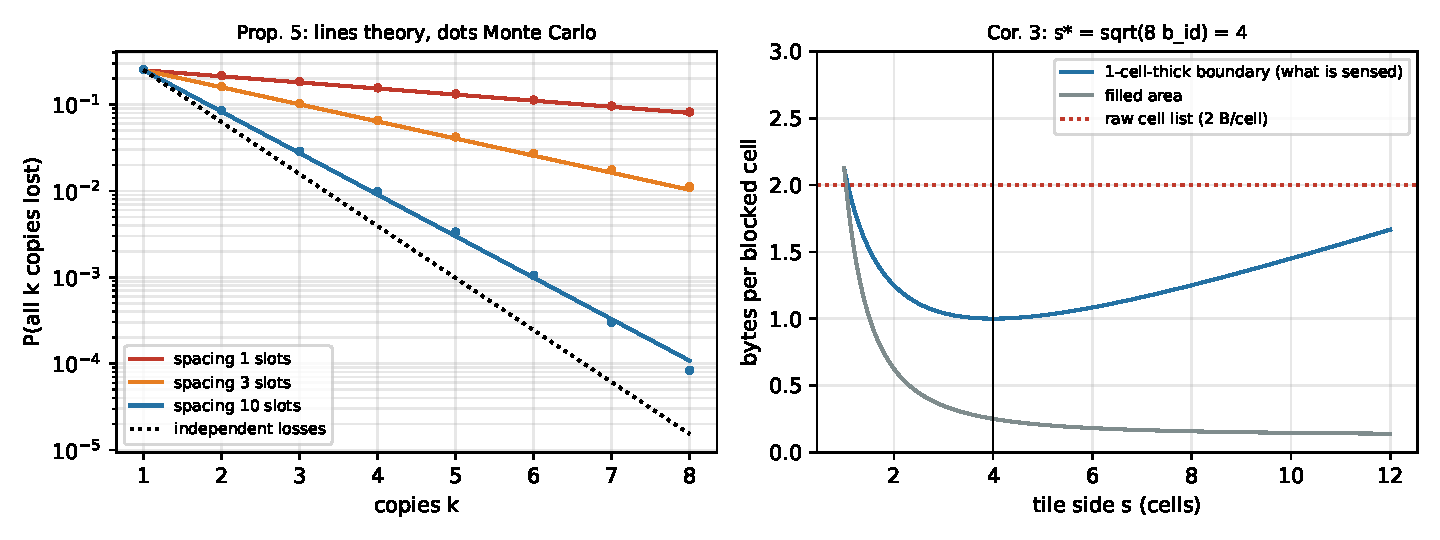
\includegraphics[width=\linewidth]{fig/theory_checks.pdf}
\caption{Left: Proposition~\ref{prop:allLost} (lines) against Monte Carlo simulation of the chain (dots), $\pi_B=0.25$, mean outage 6.7 slots. Right: bytes per blocked cell against tile side (Corollary~\ref{cor:tile}).}
\label{fig:theory}
\end{figure}

\paragraph{Theory checks (Figure~\ref{fig:theory}).} The closed form of Proposition~\ref{prop:allLost} matches Monte Carlo over four orders of magnitude, and shows that one-slot repetition on a bursty link barely helps. The test suite also checks Proposition~\ref{prop:cond}, $k^\star$ (Proposition~\ref{prop:kstar}) against brute force, Lemma~\ref{lem:tiles} exactly, Lemma~\ref{lem:ellipse} and Proposition~\ref{prop:voi} on random terrains, the memory bound, and that the agent code cannot import the world.


\section{Limitations and next steps}
\begin{itemize}
\item \textbf{Model:} the world is a 2-D grid with static obstacles, localisation is perfect, all agents are identical, and the link memory $\lambda$ is a fixed design constant rather than learned on board.
\item \textbf{Theory:} the ellipse prior assumes an exponential cost rise; Proposition~\ref{prop:voi} assumes the receiver detects an obstacle within path distance $r$ ahead; and with bounded memory there is no completeness guarantee.
\item \textbf{Validation:} the radio is simulated. The next step is to run the same agent code over Zenoh with \texttt{tc netem} and in PX4 SITL, as the roadmap plans, and to feed GRACE tiles to a common operational picture as Cursor on Target.
\item \textbf{Extensions:} learning $\lambda$ from loss runs; heterogeneous teams with different sensors and roles; adversarial or byzantine reports; sharing interference maps as well as obstacles.
\end{itemize}

\paragraph{Responsible use.} This is open, basic research on information-efficient coordination for dual-use applications such as search and rescue and infrastructure inspection. It uses only synthetic data and contains no weapon, targeting or vehicle-specific control code.

\begin{thebibliography}{99}\small
\bibitem{stentz94} A.~Stentz. Optimal and efficient path planning for partially-known environments. \emph{IEEE ICRA}, 1994.
\bibitem{koenig02} S.~Koenig and M.~Likhachev. D* Lite. \emph{AAAI}, 2002.
\bibitem{moravec85} H.~Moravec and A.~Elfes. High resolution maps from wide angle sonar. \emph{IEEE ICRA}, 1985.
\bibitem{howard66} R.~A.~Howard. Information value theory. \emph{IEEE Trans.\ Systems Science and Cybernetics}, 2(1):22--26, 1966.
\bibitem{gilbert60} E.~N.~Gilbert. Capacity of a burst-noise channel. \emph{Bell System Technical Journal}, 39(5):1253--1265, 1960.
\bibitem{elliott63} E.~O.~Elliott. Estimates of error rates for codes on burst-noise channels. \emph{Bell System Technical Journal}, 42(5):1977--1997, 1963.
\bibitem{shapiro11} M.~Shapiro, N.~Pregui\c{c}a, C.~Baquero and M.~Zawirski. Conflict-free replicated data types. \emph{SSS}, 2011.
\bibitem{ccopi} B.~Liu and T.~Zhang. CC-OPI: online distributed task allocation for UAV swarms under communication constraints. arXiv:2609.19208, 2026.
\bibitem{karakasis26} P.~A.~Karakasis and W.~Saad. Latent semantic state estimation for reliable swarming of UAVs under intermittent connectivity. arXiv:2608.08895, 2026.
\bibitem{zhao26} R.~Zhao et al. Don't fire together: desynchronised communication scheduling for bandwidth-limited multi-robot exploration. \emph{Sensors} 26(15):4778, 2026.
\end{thebibliography}
\end{document}
